% Juneki Hong and Michael Tango
% Declarative Methods
% Professor Eisner
% May 3, 2013


\documentclass{article}
\usepackage{acl2012}
\usepackage{times}
\usepackage{latexsym}
\usepackage{amsmath}
\usepackage{multirow}
\usepackage{url}
\usepackage{tikz}

\usepackage[english]{babel}
\usepackage{graphicx}
\setlength\titlebox{6.5cm}    % Expanding the titlebox


\title{Declarative Methods Term Project: \\ JumanG}
\author{Juneki Hong and Michael Tango}

%\usepackage[ampersand]{easylist}

\date{}
\begin{document}
\maketitle

\begin{abstract}
In this paper we introduce JumanG, a system that will attempt to display graphs in an effective or aesthetically pleasing way. We implement several types of familiar graph layout methods, and then given a graph we perform some analysis to attempt to decide which method to perform. We will compare the results of our implemented graph layout methods to the results of similar GraphViz layout programs, and we will show how our display decision process automatically handles a variety of graphs appropriately.
\end{abstract}

\section{Introduction}
Graphs can represent a wide range of data and information, and the task of visualizing graphs is important in revealing the patterns and underlying structure within them. Although many heuristics are available for what determines a "good" visualization such as number of edge crossings, regular spacing, and node overlaps, in the end the best way to visualize a given graph might be circumstantial or domain specific. 
There are subsequently several specialized layout methods that can perform well in particular instances for effective or aesthetic display.
 
Programs such as GraphViz have several different layout methods, but this relies on the user to decide which one to use. 
In other words, the user is required to have an intuition about how each solver works and would make their graph appropriately look the best. Instead of having the user say \textit{how} the graph should be displayed, we intend to let the user express only that a graph should be displayed.

JumanG seeks to determine which layout method is most appropriate by doing some analysis on some features of the graph such as its size, directedness, branching factor, and cyclicity.

\section{The JumanG Pipeline}
The JumanG system has three main sections in its pipeline. It has an \textit{encoder} that parses in a graph specification into its internal data structures, a set of \textit{solvers} that will lay out the graph and assign coordinate values to display, and a \textit{decoder} that takes the processed graph and outputs out to Tikz LaTeX where it can be displayed on the screen.

\subsection{The Encoder and the Dot Language}
The encoder for JumanG starts by reading in a Dot file. 
Dot is a Little Language used for the specification of graphs, and so we wanted to use Dot files as a graph description for which we could parse in and process.
We built a parser that accomplishes this, passing off the internal graph to our solvers.


\subsection{Analysis and Solvers}
We implemented several different graph layout solvers (as well as call one from GraphViz). These solvers all implement previous well known layout methods. They work well in different situations, and JumanG attempts to decide which of these would be the best to use.

In order to do this, JumanG decides based on the features extracted. Directed acyclic graphs would be run with the Layered Solver, directed and undirected graphs with very high branching factor would be run with our Radial Solver, directed rings would be run with the GraphViz Circo Solver, and all other undirected graphs and graph meshes would be run with our Springs Solver. 

In this way, we formed a Decision Tree that would allow JumanG's analysis to determine which solver to run the given graph against.



\begin{figure}
\caption{Radial Solver on a graph with high branching factor}
\label{sprawl}
\begin{tikzpicture}[scale=0.40, transform shape]
	\tikzstyle{every node} = [circle, fill=gray!30, minimum size = 1.4cm]
	\node (24) at (3.52, 8.28) {24};
	\node (25) at (1.25, 8.91) {25};
	\node (26) at (-8.34, -3.37) {26};
	\node (27) at (-7.55, -4.90) {27};
	\node (20) at (1.55, -5.80) {20};
	\node (21) at (3.86, -4.60) {21};
	\node (22) at (5.20, -3.00) {22};
	\node (23) at (5.91, -1.04) {23};
	\node (28) at (-6.89, -5.79) {28};
	\node (29) at (7.19, -5.42) {29};
	\node (1) at (0.00, 0.00) {1};
	\node (3) at (0.00, 3.00) {3};
	\node (2) at (2.60, 1.50) {2};
	\node (5) at (-2.60, -1.50) {5};
	\node (4) at (-2.60, 1.50) {4};
	\node (7) at (2.60, -1.50) {7};
	\node (6) at (0.00, -3.00) {6};
	\node (9) at (5.56, 2.25) {9};
	\node (8) at (5.96, 0.73) {8};
	\node (11) at (3.69, 4.73) {11};
	\node (10) at (4.79, 3.61) {10};
	\node (13) at (-1.55, 5.80) {13};
	\node (12) at (1.55, 5.80) {12};
	\node (15) at (-5.96, -0.73) {15};
	\node (14) at (-5.20, 3.00) {14};
	\node (17) at (-4.79, -3.61) {17};
	\node (16) at (-5.56, -2.25) {16};
	\node (19) at (-1.55, -5.80) {19};
	\node (32) at (8.86, -1.56) {32};
	\node (31) at (8.16, -3.80) {31};
	\node (30) at (7.71, -4.64) {30};
	\node (18) at (-3.69, -4.73) {18};
	\draw [->] (22)--(29);
	\draw [->] (22)--(30);
	\draw [->] (22)--(31);
	\draw [->] (23)--(32);
	\draw [->] (1)--(2);
	\draw [->] (1)--(3);
	\draw [->] (1)--(4);
	\draw [->] (1)--(5);
	\draw [->] (1)--(6);
	\draw [->] (1)--(7);
	\draw [->] (3)--(12);
	\draw [->] (3)--(13);
	\draw [->] (2)--(8);
	\draw [->] (2)--(9);
	\draw [->] (2)--(10);
	\draw [->] (2)--(11);
	\draw [->] (5)--(15);
	\draw [->] (5)--(16);
	\draw [->] (5)--(17);
	\draw [->] (5)--(18);
	\draw [->] (4)--(14);
	\draw [->] (7)--(21);
	\draw [->] (7)--(22);
	\draw [->] (7)--(23);
	\draw [->] (6)--(19);
	\draw [->] (6)--(20);
	\draw [->] (12)--(24);
	\draw [->] (12)--(25);
	\draw [->] (17)--(27);
	\draw [->] (17)--(28);
	\draw [->] (16)--(26);
\end{tikzpicture}
\end{figure}



\subsection{Radial Solver}


Radial displays have been used to display trees in a way different from a typical top-down approach.
Introduced in 1991 by Eades \cite{Eades:91} %~\cite{freeTrees}, 
this layout places the branches circularly around the root outwards, drawing 
nodes at different radii from the center. We implemented our own Radial solver that uses similar techniques to the original
method. We wrote our solver to evenly distribute nodes around the root at each level, rather than the typical style of weighting 
the nodes based on the subnodes. We also chose to display nodes at their closest level to root. 
This allows the solver to draw non-tree graphs fairly well. In some instances, we can even beat Graphviz's twopi instantiation, detailed below in our experimental comparison section. %TODO wording

A radial solver can be used rather than a standard layered solver for drawing graphs that are much wider than they are deep. Our metric 
for determining whether the radial solver should be used is given by a measure of width: 
$$width = \frac{|nodes|}{depth_{graph}}$$

You can see a graph drawn using our radial solver in Figure~\ref{sprawl}.






\subsection{Springs solver}

The Springs algorithm, as outlined by Kawai and Kamada \cite{Kamada:89}, computes a layout for a graph by running a physics simulation on the graph. All of the nodes are set to repel each other, while the edges are set as ``springs" to hold the nodes together. Our solver scales the repelling forces of the nodes based on how densely connected the graphs are, in order to prevent nodes being spaced too close or far apart in the end.

This was the repulsion force used in our Springs solver:
$$ f_r = \frac{|edges|}{|nodes|}^3 \frac{1}{d^2} $$
Where d is the euclidean distance between any two nodes. 

We defined the attraction function between two connected nodes as a linear factor of the distance between two nodes. With the constraints in place the simulation attempts to minimize the total energy in the graph.

\subsubsection{Springs solver's Initialization}
The Springs solver also requires the nodes to have an initial configuration. Wilkinson suggests two possible approaches \cite{Wilkinson:05}. The first being random placement, where all of the nodes are randomized, and the second being based on geodesic distance. We have implemented both options, the second option using the Radial solver as an alternative to this geodesic distance initialization. 

The Radial initialization works well for graphs with sparse connections, spreading the nodes out, and giving the Springs algorithm a good starting point to begin minimizing the energy in the system. More densly connected graphs do not work as well using this, and so we default back to random jitter perturbation initialization.

We measured connectivity as:
$$connectivity = \frac{|nodes|}{|edges|}$$
Based on empirical testing we determined to use randomized initialization on graphs with connectivity higher than 3.


\begin{figure}
\caption{A Sparsely Connected Graph with the Springs Solver with Radial Initialization}
\begin{tikzpicture}[scale=0.40, transform shape]
	\tikzstyle{every node} = [circle, fill=gray!30, minimum size = 1.8cm]
	\node (H4) at (0.16, -4.08) {H4};
	\node (H5) at (-5.44, -2.10) {H5};
	\node (H2) at (3.43, 8.65) {H2};
	\node (H3) at (-4.62, 3.79) {H3};
	\node (H0) at (8.17, 0.76) {H0};
	\node (H1) at (9.03, 6.64) {H1};
	\node (C1) at (-1.14, 0.52) {C1};
	\node (C0) at (4.71, 4.05) {C0};
	\draw [-] (H4)--(C1);
	\draw [-] (H5)--(C1);
	\draw [-] (H2)--(C0);
	\draw [-] (H3)--(C1);
	\draw [-] (H0)--(C0);
	\draw [-] (H1)--(C0);
	\draw [-] (C1)--(C0);
	\draw [-] (C1)--(H3);
	\draw [-] (C1)--(H4);
	\draw [-] (C1)--(H5);
	\draw [-] (C0)--(H0);
	\draw [-] (C0)--(H1);
	\draw [-] (C0)--(H2);
	\draw [-] (C0)--(C1);
\end{tikzpicture}
\end{figure}



\begin{figure}
\caption{A Densely Connected Graph with the Springs Solver with Random Jitter Initialization}
\begin{tikzpicture}[scale=0.70, transform shape]
	\tikzstyle{every node} = [circle, fill=gray!30, minimum size = 1.8cm]
	\node (k3) at (0.72, 3.87) {k3};
	\node (k2) at (-3.06, -2.52) {k2};
	\node (k1) at (1.41, -3.52) {k1};
	\node (k5) at (-3.49, 2.05) {k5};
	\node (k4) at (3.75, 0.43) {k4};
	\draw [-] (k3)--(k1);
	\draw [-] (k3)--(k2);
	\draw [-] (k3)--(k4);
	\draw [-] (k3)--(k5);
	\draw [-] (k2)--(k1);
	\draw [-] (k2)--(k3);
	\draw [-] (k2)--(k4);
	\draw [-] (k2)--(k5);
	\draw [-] (k1)--(k2);
	\draw [-] (k1)--(k3);
	\draw [-] (k1)--(k4);
	\draw [-] (k1)--(k5);
	\draw [-] (k5)--(k1);
	\draw [-] (k5)--(k2);
	\draw [-] (k5)--(k3);
	\draw [-] (k5)--(k4);
	\draw [-] (k4)--(k1);
	\draw [-] (k4)--(k2);
	\draw [-] (k4)--(k3);
	\draw [-] (k4)--(k5);
\end{tikzpicture}
\end{figure}


\subsection{Layered Solver}
Layered graph, or Sugiyama-style drawing is an approach to arranging directed acyclic graphs \cite{Sugiyama:81}. This drawing approach relies on assigning the nodes to a ``layer" in the graph and then assigning descending y-coordinates for each successive layer from the root. Then, for each layer, the nodes are rearranged to minimize the edge crossings in between layers.

Our implementation of a Layered Solver assigns its layers determined by a ``topological ordering" starting with the root nodes of the DAG. We topologically sort the graph, but all of the nodes are marked with the iteration at which they were added to the sorted list. 

After determining all of the layers, the nodes in each layer are rearranged in an attempt to minimize edge crossings. Determining an ordering that minimizes edge crossings is NP-Complete \cite{Eades:94}, and so we rely on heuristics to accomplish this task.

\begin{figure}
\caption{A Directed Acyclic Graph with the Layered Solver}
\begin{tikzpicture}[scale=0.70, transform shape]
	\tikzstyle{every node} = [circle, fill=gray!30, minimum size = 1.8cm]
	\node (a) at (0.00, 0.00) {a};
	\node (c) at (1.50, -3.00) {c};
	\node (b) at (-1.50, -3.00) {b};
	\node (e) at (3.00, -6.00) {e};
	\node (d) at (-3.00, -6.00) {d};
	\node (f) at (0.00, -6.00) {f};
	\node (c2) at (4.50, -3.00) {c2};
	\node (c1) at (-4.50, -3.00) {c1};
	\draw [->] (a)--(b);
	\draw [->] (a)--(c);
	\draw [->] (a)--(c1);
	\draw [->] (a)--(c2);
	\draw [->] (c)--(e);
	\draw [->] (c)--(f);
	\draw [->] (b)--(d);
	\draw [->] (b)--(e);
	\draw [->] (b)--(f);
	\draw [->] (b)--(d);
	\draw [->] (c2)--(e);
	\draw [->] (c1)--(d);
\end{tikzpicture}
\end{figure}



\subsubsection{Edge Crossing Minimization Heuristic}
The heuristic our Layered Solver used to order nodes and minimize edge crossings between layers relies on a calculation analogous to ``center of mass" using the edges between the surrounding layers. Each node is assigned an averaged index interpolating between the indexes of all the adjacent nodes above and below the layer, and then the nodes are sorted based on these indexes. 


\begin{figure}
\caption{Edge Crossing Heuristic Illustration}\label{layers}
\centering
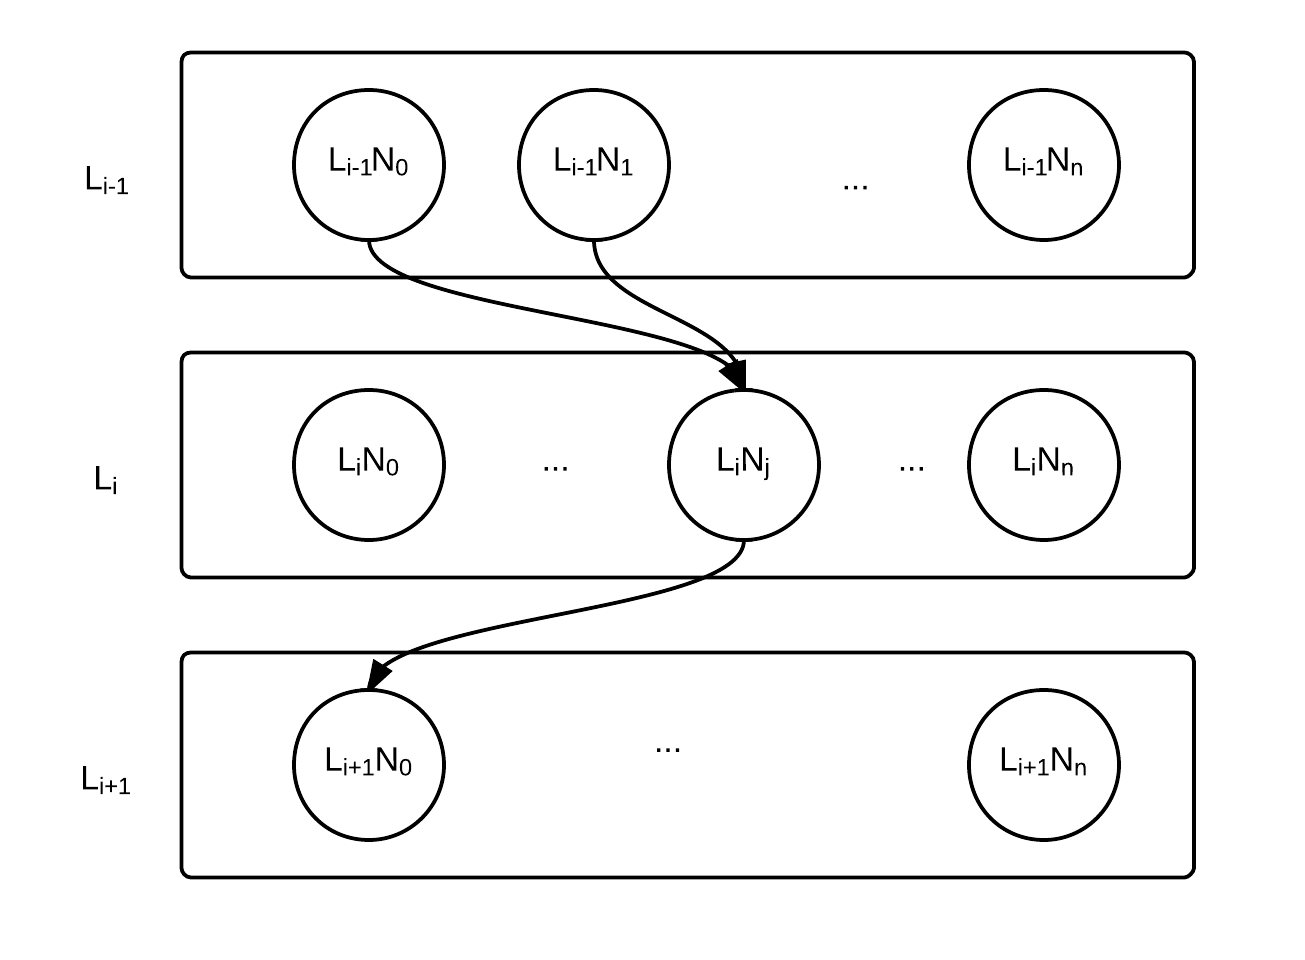
\includegraphics[width=0.52\textwidth]{layereddia.png}
\end{figure}

From Figure~\ref{layers}, our index calculations are as such.

$$ index(L_i , n_j) = \frac{\sum\limits_a index(L_{i-1}n_a) + \sum\limits_b index(L_{i+1}n_b)}{|L_{i-1}n_a| + |L_{i+1}n_b|}$$
$$\forall Edge(n_a , n_j), Edge(n_j , n_b)$$
This heuristic is greedy in that at each layer we try to place nodes closer to its adjacent nodes.




\subsection{Circo Solver}
Circo is a graph layout solver available from within GraphViz that specializes in arranging circular graphs. 
We use Circo as one of our available graph solvers because we did not implement our own version of a circular layout solver.

%TODO put in an example picture
\begin{figure}[h!]
\caption{A Ring Graph solved by the Circo Solver}
\centering
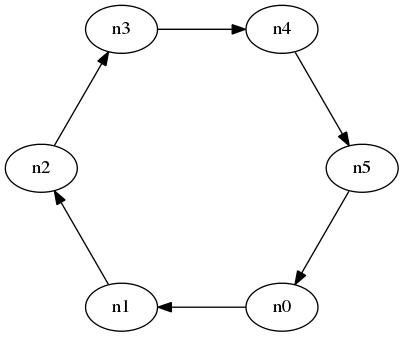
\includegraphics[width=0.3\textwidth]{circo.jpg}
\end{figure}

In our analysis of the given graph, we can determine that a graph is a directed cycle if there are no root nodes, that is nodes that do not have inward edges pointing to them. When a graph is a directed cycle, the Circo Solver tends to have good results. 

For undirected cycles, our Spring Solver does a good job because the edges ``pull" in both directions, and so the balanced forces can properly work on the simulation. In JumanG, we use our Spring Solver when we detect such undirected cycles. 

%\begin{figure}
%\caption{The same Undirected Ring Graph solved by the Springs Solver}
%\begin{tikzpicture}[scale=0.40, transform shape]
%	\tikzstyle{every node} = [circle, fill=gray!30, minimum size = 1.8cm]
%	\node (n0) at (-0.17, -0.79) {n0};
%	\node (n1) at (-0.17, 4.10) {n1};
%	\node (n2) at (4.06, 6.54) {n2};
%	\node (n3) at (8.30, 4.09) {n3};
%	\node (n4) at (8.30, -0.80) {n4};
%	\node (n5) at (4.06, -3.24) {n5};
%	\draw [-] (n0)--(n1);
%	\draw [-] (n0)--(n5);
%	\draw [-] (n1)--(n0);
%	\draw [-] (n1)--(n2);
%	\draw [-] (n2)--(n1);
%	\draw [-] (n2)--(n3);
%	\draw [-] (n3)--(n2);
%	\draw [-] (n3)--(n4);
%	\draw [-] (n4)--(n3);
%	\draw [-] (n4)--(n5);
%	\draw [-] (n5)--(n4);
%	\draw [-] (n5)--(n0);
%\end{tikzpicture}
%\end{figure}


\subsection{The Decoder: TikZ}
After our analysis for choosing the solver and after running the chosen solver, JumanG outputs the processed graph out to TikZ LaTeX. TikZ is a graphics package we could manipulate directly to draw the nodes and edges at all the specified coordinates to represent the graph.

By default, the decoder creates the output file that fills out an entire page of a document. The examples embedded in this paper have been scaled down.




\section{Experimental Comparison}

\begin{figure}[h!]
\caption{GraphViz's neato solver's version of a Sierpinski triangle}
\label{neatoSierpinski}
\centering
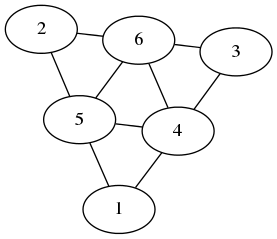
\includegraphics[width=0.3\textwidth]{serp.png}
\end{figure}

\begin{figure}
\caption{Our Spring Solver's version of a Sierpinski triangle}
\label{springSierpinski}
\begin{tikzpicture}[scale=0.40, transform shape]
	\tikzstyle{every node} = [circle, fill=gray!30, minimum size = 1.8cm]
	\node (1) at (4.55, -4.87) {1};
	\node (3) at (-6.33, -1.86) {3};
	\node (2) at (1.72, 6.06) {2};
	\node (5) at (2.95, 0.54) {5};
	\node (4) at (-0.84, -3.18) {4};
	\node (6) at (-2.16, 1.96) {6};
	\draw [-] (1)--(4);
	\draw [-] (1)--(5);
	\draw [-] (3)--(4);
	\draw [-] (3)--(6);
	\draw [-] (2)--(5);
	\draw [-] (2)--(6);
	\draw [-] (5)--(1);
	\draw [-] (5)--(2);
	\draw [-] (5)--(4);
	\draw [-] (5)--(6);
	\draw [-] (4)--(1);
	\draw [-] (4)--(3);
	\draw [-] (4)--(5);
	\draw [-] (4)--(6);
	\draw [-] (6)--(2);
	\draw [-] (6)--(3);
	\draw [-] (6)--(4);
	\draw [-] (6)--(5);
\end{tikzpicture}
\end{figure}

In many cases, our graph layout solvers perform comparatively to Graphviz solvers. For example, in Figure~\ref{neatoSierpinski} we show GraphViz's ``neato" Spring Solver, compared to Figure~\ref{springSierpinski}. We render a Sierpinski triangle, automatically choosing the Springs solver with random jitter initialization.


\begin{figure}[h!]
\caption{GraphViz's 2Pi Radial Solver's version of an example graph}
\label{twopiTurnip}
\centering
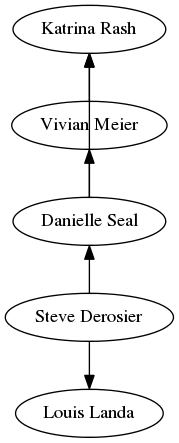
\includegraphics[width=0.15\textwidth]{turnip_dag.png}
\end{figure}

\begin{figure}
\caption{Our Radial Solver's version of the example graph. Compared to 2Pi.}
\label{radialTurnip}
\begin{tikzpicture}[scale=0.60, transform shape]
	\tikzstyle{every node} = [circle, fill=gray!30, minimum size = 1.8cm]
	\node (Steve) at (0.00, 0.00) {Steve};
	\node (Louis) at (0.00, -3.00) {Louis};
	\node (Katrina) at (-4.24, 4.24) {Katrina};
	\node (Danielle) at (0.00, 3.00) {Danielle};
	\node (Vivian) at (4.24, 4.24) {Vivian};
	\draw [->] (Steve)--(Danielle);
	\draw [->] (Steve)--(Louis);
	\draw [->] (Danielle)--(Vivian);
	\draw [->] (Danielle)--(Katrina);
	\draw [->] (Vivian)--(Katrina);
\end{tikzpicture}
\end{figure}


In some cases, JumanG's solvers displayed graphs more effectively than comparable GraphViz solvers, as in Figure~\ref{twopiTurnip} and in Figure~\ref{radialTurnip}.




\section{Future Work}
JumanG could be extended in a variety of ways that may be interesting. 

\subsection{Learned Analysis Parameters}
Instead of developing the solver decision tree by hand, we could try to learn parameters that determine which graph layouts are more favorable than others. 

Using our graph analysis toolkit, we can extract a set of features of a graph such as its size, directedness, and branching factor. We could also go expand this and have additional features such as the strongly connected components, diameter, or bipartiteness.

We could learn which parameters determine which graph layouts are the best. We could generate a large set of random graphs, and process all of them with each of our graph layout solvers. We could get annotated data by using a service like Mechanical Turk, presenting every solver's representation of each graph side-by-side and asking the users to choose the graph layout the best visualizes the data.

Using the analysis features, we could develop a multi-class classifier to learn which graph layouts are the best for any arbitrary graph.


\subsection{Handling and Displaying more Dot Features}
This project was primarily focused on graph layout, but the Dot Language can support much richer features such as edge labels, node labels, and node colors. Further work could include expanding our parser to handle anything within the Dot Language. We could also allow the user to set the positions of some of the nodes and then solve around them.


\subsection{Additional Solvers}
On a basic level, more solvers could be implemented and the analysis could further developed be used to choose among them. Additional Solvers might handle arranging graphs in N-dimensions, and the analysis could determine to use such a solver if the graph was sufficiently non-planar.



\section{Conclusion}
Graph drawing can be difficult due to its underspecified nature. Across different users and domains there can be varying expectations and requirements. In this respect, trying to effectively represent any graph for any user might be intractible. However, JumanG attempts to handle this task anyway, achieving some good results on a variety of inputs. It does this by determining which layout is most appropriate to the input graph.



%\bibliographystyle{plain}
%\bibliography{citations}
\begin{thebibliography}{}

%springs
\bibitem[\protect\citename{Kamada and Kawai}1989]{Kamada:89}
Tomihisa Kamada and Satoru Kawai.
\newblock 1989.
\newblock {\em An Algorithm for Drawing General Undirected Graphs}, volume~31.
\newblock Information Processing Letters.

%grammerGraphics
\bibitem[\protect\citename{Wilkinson}2005]{Wilkinson:05}
Leland Wilkinson
\newblock 2005.
\newblock {\em The Grammar of Graphics}.
\newblock Springer Science+Business Media, Inc.

%radial
\bibitem[\protect\citename{Eades}1991]{Eades:91}
Peter Eades
\newblock 1991.
\newblock {\em Drawing Free Trees}.
\newblock International Institute for Advanced Study of Social Information Science, Fujitsu Limited.

% edgecrossings is NP
\bibitem[\protect\citename{Eades}1994]{Eades:94}
Eades, Peter and Wormald, Nicholas C.
\newblock 1994.
\newblock {\em Edge crossings in drawings of bipartite graphs}, volume~11.
\newblock Springer-Verlag.

%layered
\bibitem[\protect\citename{Sugiyama}1981]{Sugiyama:81}
Kozo Sugiyama
\newblock 1981.
\newblock {\em Methods for Visual Understanding of Hierarchical System Structures}, volume~11.
\newblock IEEE Transactions on Systems, Man, and Cybernetics.









\end{document}
